\chapter{Marco te\'orico}\label{chapter:state-of-the-art}

\par Durante la d\'ecada de los 70, un grupo relativamente pequeño de investigadores se involucró en el tema tratando al análisis de imágenes m\'edicas como un problema de procesamiento de información en una única imagen. Esta l\'inea posee enfoques basados en reconocimiento de patrones, procesamiento de imágenes y/o señales y visión computarizada. En 1973, Sklansky y Ballard [\cite{1}] describen un m\'etodo por el cual una computadora realza los bordes de las imágenes de tumores en radiografías y escaneo de isótopos. El algoritmo extendido detecta el mejor conjunto de curvas cerradas localmente convexas que contienen candidatos a tumores. Por lo tanto, se desarrolló una técnica de selección con criterios subjetivos para clasificar a los candidatos y seleccionar los que probablemente fueran tumores. Seg\'un los investigadores, aunque la naturaleza de la imagen de datos dificultó la mejora de los bordes debido a la tecnolog\'ia de esta \'epoca, se obtuvieron resultados positivos.

\par Otros esfuerzos, como el trabajo de Pizer y Todd-Pokropek [\cite{2}] en 1978, enfatizaron el mejoramiento de la imagen y las estrategias de visualización usando t\'ecnicas lineales y estacionarias para corregir el ruido y la degradaci\'on, observando que estos eran problemas críticos para los usuarios finales (radiólogos y otros). Si bien no clasifican ni automatizan la detecci\'on de anomal\'ias, estas t\'ecnicas sentaron las bases del preprocesamiento.

\par Hacia la d\'ecada de 1980, se realizaron varias investigaciones cuya caracter\'istica fundamental fue el desarrollo de ideas que se basaban en la detecci\'on de bordes por contraste en bancos de datos bidimensionales y, luego, la aplicaci\'on de un agrupamiento o uni\'on b\'asica de bordes utilizando algún tipo de heurística de búsqueda de contorno, basándose en las propiedades de suavidad de la imagen a analizar, tal y como se expone en el trabajo de Yachida [\textcolor{cyan}{\cite{3}}] de 1980. Estos enfoques aprovecharon algunos avances generales hechos por la comunidad científica orientada al procesamiento de imágenes y visión computarizada, y podría ser visto como el precursor de la variedad de enfoques de búsqueda de bordes deformables presentes en el desarrollo de hoy en día.

\par Los primeros intentos de sistemas de dise\~no asistido por computadora (CAD, en ingl\'es) completamente automático en mamografías de rayos X fueron propuestos sobre 1987 (Chan et al [\textcolor{cyan}{\cite{4}}]). En el mismo se investig\'o la aplicaci\'on de algoritmos para la detecci\'on de microcalcificaciones en mamograf\'ias digitales. El sistema de detecci\'on de la anomal\'ia se bas\'o en una t\'ecnica de diferenciaci\'on entre una imagen con se\~nal suprimida y una imagen con se\~nal mejorada para eliminar el fondo estructurado en la mamografía. Para ello, se emple\'o el m\'etodo de Monte Carlo, con el fin de generar grupos de microcalcificaciones que se superponen en el fondo de la mamograf\'ia. Esto permiti\'o una evaluación de la precisión de detección del método y la dependencia de esta precisión de las características físicas de las microcalcificaciones.

\par Como parte del proceso de mejoramiento de la imagen, se emple\'o un filtro espacial que estuviese correlacionado con el tama\~no y caracter\'isticas de la microcalcificaci\'on. Aunque no es un tema que se expuso directamente en la investigaci\'on, se comenz\'o a desarrollar la idea del uso de wavelets para la detecci\'on de anomal\'ias, lo que dio paso a que, en los inicios del siglo actual, se comenzaran a realizar nuevos proyectos de procesamiento digital empleando las funciones wavelets.

\par En 2005, Jos\'e Salvado y Bruno Roque [\textcolor{cyan}{\cite{5}}] publican un art\'iculo sobre el uso del an\'alisis wavelet para la detecci\'on de calcificaciones en mamograf\'ias digitales. Se aplica el concepto de filtro, descomposici\'on y reconstrucci\'on de la imagen caracter\'istico de las wavelets, a fin de eliminar el ruido en la mamograf\'ia digital y obtener una muestra mejorada que permita una detecci\'on efectiva de la anomal\'ia.

\par Muchos son los algoritmos que se han desarrollado para el procesamiento de im\'agenes y detecci\'on de patrones que hacen uso de t\'ecnicas de aprendizaje autom\'atico, sin embargo, el empleo de wavelets para la detecci\'on de patrones es una t\'ecnica que no se ha explotado lo suficiente en comparaci\'on al m\'etodo anterior, a lo que salta la pregunta, ?`qu\'e son las wavelets y c\'omo podr\'ian usarse en la detecci\'on de patrones?

\section{Introducci\'on a las Wavelets}

\par El origen de la teor\'ia wavelet se remonta al an\'alisis arm\'onico del campo de las matem\'aticas puras, desarrollado por el matem\'atico franc\'es Jean Baptiste Joseph Fourier (1768-1830), conocido por ser el primero en crear un m\'etodo para expresar toda funci\'on peri\'odica como suma de funciones trigonom\'etricas (senos y cosenos) llamada Series Trigonom\'etricas de Fourier.

\par A inicios del siglo XX, Alfred Haar desarroll\'o un conjunto de funciones que m\'as adelente se nombrar\'ian en su honor: Wavelets de Haar. Estas constituyen el caso m\'as simple conocido de funciones wavelets y pueden ser utilizadas para el an\'alisis de una se\~nal en tiempo y frecuencia, debido a la propiedad que tienen de tener una mayor localizaci\'on que las funciones arm\'onicas utilizadas en el an\'alisis de Fourier.

\par M\'as tarde, Paul Levy (1886-1971) demostr\'o que las Wavelets de Haar, debido a su propiedad de escalado, brindan una mejor forma de modelar las funciones que el an\'alisis de Fourier [\textcolor{cyan}{\cite{6}}].

\par En 1984, Jean Morlet [\cite{21}] en su intento de ayudar a los ge\'ologos franceses para encontrar herramientas m\'as efectivas de localizaci\'on de petr\'oleo, desarroll\'o una forma de analizar las se\~nales s\'ismicas para crear componentes que estuviesen bien localizadas en el espacio, llam\'andolas onditas, que m\'as tarde ser\'ian conocidas como las wavelets de Morlet.

\par Hacia 1986 y 1987, la demostraci\'on de que la teor\'ia wavelets aparece impl\'icita en el an\'alisis multirresoluci\'on por parte de Stéphane Mallat en 1986 y el descubrimiento en 1987 de Ingrid Daubechies de una nueva clase de wavelet que no solo era ortogonal sino que pod\'ia ser implementada usando ideas de filtrado digital simple, provocaron el detonante en la revoluci\'on wavelet [\textcolor{cyan}{\cite{7}}].

\subsection{Definiciones}

\par La palabra wavelet significa onda peque\~na u ondita. Matem\'aticamente quiere decir que la onda es de corta duraci\'on; esta caracter\'istica se conoce como localizaci\'on y es una de las ventajas que proporcionan las funciones wavelets sobre la serie de Fourier, Figura~\ref{wav-fourier}.\\

\begin{figure}[h]
\center
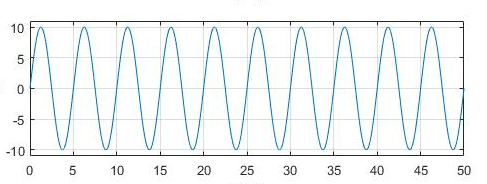
\includegraphics[height=29mm, width=45mm]{Graphics/FourierOnda.png}
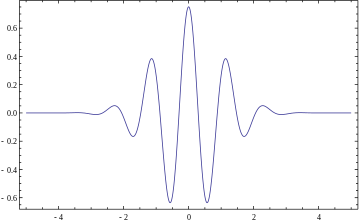
\includegraphics[scale=.33]{Graphics/FuncionWavelet.png}
\caption{Izquierda: Onda (Fourier). Derecha: Ondita (Wavelet).}
\label{wav-fourier}
\end{figure}

\begin{definition}
De manera formal, una wavelet es una funci\'on $\Psi(t)\in L^2(\mathbb{R})$ tal que la familia de funciones:
\begin{eqnarray}
\Psi_{a,b}(t)&:=&\frac{1}{\sqrt{a}}\Psi\left(\frac{t-b}{a}\right),\nonumber
\end{eqnarray}
donde $a$ y $b$ son reales que indican la escala y el desplazamiento, respectivamente, es una base ortonormal en el espacio de Hilbert $L^2(\mathbb{R})$.
\label{wav-continua}
\end{definition}

\par Este conjunto de funciones est\'an definidas en todo $\mathbb{R}$, por lo que representan funciones continuas, para los intervalos en los cuales se definen. Aunque esta forma de expresar las definici\'on de funciones wavelets es muy \'util para el an\'alisis, fundamentalmente te\'orico, de se\~nales en investigaciones cient\'ificas, puede presentar un problema para la codificaci\'on de las mismas en campos como la ingenier\'ia y las ciencias computacionales. Por ello, se define el espacio $\ell^2\left(\mathbb{Z}_N\right)=\{z(i)|0\leq i \leq N-1\}$ donde $z$ representa un vector de dimensi\'on $N$, en el cual se brindar\'a una definici\'on discreta, m\'as tratable para equipos de c\'omputo y ser\'a la que se utilizar\'a en lo adelante.\\

\begin{definition}
Se define la funci\'on wavelet discreta $\Psi(t)\in \ell^2(\mathbb{Z}_N)$ tal que la familia de funciones:
\begin{eqnarray}
\Psi_{j,k}(t)&:=&2^{\frac{j}{2}}\Psi(2^jt-k),\nonumber
\end{eqnarray}
con $j$ y $k$ enteros, es una base ortonormal en el espacio $\ell^2(\mathbb{Z}_N)$.
\label{wav-discreta}
\end{definition}

\par Como se puede apreciar, la definici\'on de wavelet discreta se obtiene al discretizar los parámetros de desplazamiento y escalamiento dentro de la definici\'on de wavelet continua:
\begin{eqnarray}
a&=&2^{-j}\nonumber\\
b&=&k2^{-j}\qquad\mbox{con $j,k\in \mathbb{Z}$}.\nonumber
\end{eqnarray}

\par A la funci\'on $\Psi$ se le llama entonces wavelet madre. En su forma discreta, cada elemento de la base wavelet constituye un vector de dimensi\'on $N$. Se ver\'a entonces c\'omo es posible obtener esta base y, por tanto, wavelet madre. A continuaci\'on se presentan un conjunto de definiciones a fin de proporcionar una notaci\'on y un algoritmo para obtener dichas wavelets.\\

\begin{definition}
Se define la transformada discreta de Fourier del vector $w\in \ell^2\left(\mathbb{Z}_N\right)$ como:
\begin{eqnarray}
\hat{w}(m)=\sum_{n=0}^{N-1}w(n)e^{\frac{-2\pi imn}{N}},\quad\forall\,m\nonumber
\end{eqnarray}
\end{definition}

\begin{definition}
Se define la reflexi\'on conjugada $\tilde{w}$ de un vector $w\in \ell^2\left(\mathbb{Z}_N\right)$ como:
\begin{eqnarray}
\tilde{w}(n)=\overline{w(-n)}=\overline{w(N-n)}.\nonumber
\end{eqnarray}
\end{definition}

\begin{definition}
Se define la convoluci\'on $\ast$ entre dos vectores $w,z\in \ell^2(\mathbb{Z}_N)$ como:
\begin{eqnarray}
(z \ast w )(n) = \sum_{i=0}^{N-1}w(i)z(n-i).\nonumber
\end{eqnarray}
\end{definition}

\begin{definition}
Sea $w\in \ell^2(\mathbb{Z}_N)$ un vector y $k\in\mathbb{Z}$, se define $R_kw$ como la traslaci\'on de $w$ por $k$ dada por:
\begin{eqnarray}
R_kw(n)=w(n-k).\nonumber
\end{eqnarray}
\end{definition}

\subsection{Banco de Filtros}

\begin{definition}
Sea $N$ divisible por $2^p$. Se define un banco de filtros wavelet de $p$ escalas a partir de dos sucesiones de vectores $u_1$, $u_2$, ..., $u_p$ y $v_1$, $v_2$, ..., $v_p$, tales que:
\begin{eqnarray}
u_j, v_j \in \ell^2 \left(\mathbb{Z}_{\frac{N}{2^{j-1}}}\right),~\forall\,j=1,2,\cdots,p,\nonumber
\end{eqnarray}
y tales que la matriz del sistema:
\begin{eqnarray}
A_j(m) = \frac{1}{\sqrt{2}}\left[\begin{array}{cc}
\hat{u}_j(m)&\hat{v}_j(m)\\
\hat{u}_j\left(m+\frac{N}{2^j}\right)&\hat{v}_j\left(m+\frac{N}{2^j}\right)
\end{array}\right],\nonumber
\end{eqnarray}
es unitaria $\forall\,m=0,1,\cdots,\frac{N}{2^j}-1,\,j=1,2,\cdots,p$.
\label{banco-filtro}
\end{definition}

\par Consid\'erese esta \'ultima definici\'on. Sea $u_j\in \ell^2\left(\mathbb{Z}_{\frac{N}{2^{j-1}}}\right)$ un vector tal que $\{R_{2k}u_j\}_{k=0}^{\frac{N}{2^j}-1}$ constituye una base ortonormal. Si se define $v_j\in \ell^2\left(\mathbb{Z}_{\frac{N}{2^{j-1}}}\right)$ tal que:
\begin{eqnarray}
v_j(n)=(-1)^{n-1}\overline{u_j(1-n)},\nonumber
\end{eqnarray}
entonces, se cumple que $\{R_{2k}u_j\}_{k=0}^{\frac{N}{2^j}-1} \cup \{R_{2k}v_j\}_{k=0}^{\frac{N}{2^j}-1}$ es una base wavelet en $\ell^2\left(\mathbb{Z}_{\frac{N}{2^{j-1}}}\right)$ y, por tanto, la matriz del sistema $A_j(m)$ es unitaria para toda $m=0,1,\cdots,\frac{N}{2^j}-1$ (ver demostraci\'on en [\textcolor{cyan}{\cite{8}}]).\\

\begin{definition}
Suponga que $N$ es divisible por $2^p$. Se define $D^p:\ell^2\left(\mathbb{Z}_N\right)\rightarrow \ell^2\left(\mathbb{Z}_{\frac{N}{2^p}}\right)$ para $z\in \ell^2\left(\mathbb{Z}_N\right)$ como:
\begin{eqnarray}
D^p(z)(n)=z(2^pn),\qquad\mbox{para $n=0,1,\cdots,M-1$.}\nonumber
\end{eqnarray}
Al operador $D$ se le denomina operador de submuestreo.
\end{definition}

\begin{definition}
Suponga que $N$ es divisible por $2^p$. Se define $U^p: \ell^2\left(\mathbb{Z}_{\frac{N}{2^p}}\right)\rightarrow \ell^2\left(\mathbb{Z}_N\right)$ para $z\in \ell^2\left(\mathbb{Z}_{\frac{N}{2^p}}\right)$ como:
\begin{eqnarray}
U^p(z)(n)=\left\{\begin{array}{ll}
z\left(\frac{n}{2^p}\right)&\quad\mbox{si $n$ es divisible por $2^p$}\\
0&\quad\mbox{en otro caso.}
\end{array}\right.\nonumber
\end{eqnarray}
Al operador $U$ se le denomina operador de sobremuestreo.
\end{definition}

\begin{definition}
Suponga que $N$ es divisible por $2^p$. Sean $u_j,v_j\in \ell^2\left(\mathbb{Z}_{\frac{N}{2^{j-1}}}\right)$. Se definen $f_j,g_j\in \ell^2\left(\mathbb{Z}_N\right)$ como:
\begin{eqnarray}
f_j&=&g_{j-1}\ast U^{j-1}(v_j),\nonumber\\
g_j&=&g_{j-1}\ast U^{j-1}(u_j),\nonumber
\end{eqnarray}
para toda $j=2,3,\cdots,p$, donde $f_1=v_1$ y $g_1=u_1$.
\end{definition}

\par Consid\'erese ahora que los vectores $u_j$ y $v_j$ de la definici\'on anterior son tomados de tal forma que la matriz del sistema $A_j(n)$ es unitaria para toda $n=0,1,\cdots,\frac{N}{2^j}-1$. Entonces, se cumple que:
\begin{eqnarray}
\{R_{2^jk}f_j\}_{k=0}^{\frac{N}{2^j}-1}\cup\{R_{2^jk}g_j\}_{k=0}^{\frac{N}{2^j}-1},\nonumber
\end{eqnarray}
constituye una base ortonormal con $\frac{N}{2^{j-1}}$ elementos (ver demostraci\'on en [\textcolor{cyan}{\cite{8}}]).

\par Como consecuencia del resultado anterior, si se desarrolla el t\'ermino $g_{j-1}$ en cada nueva ecuaci\'on se obtiene la siguiente base de $\ell^2\left(\mathbb{Z}_N\right)$:
\begin{eqnarray}
\{R_{2k}f_1\}_{k=0}^{\frac{N}{2}-1}\cup\{R_{4k}f_2\}_{k=0}^{\frac{N}{4}-1}\cup ...\cup\{R_{2^{p}k}f_{p}\}_{k=0}^{\frac{N}{2^{p}}-1}\cup\{R_{2^{p}k}g_{p}\}_{k=0}^{\frac{N}{2^{p}}-1}.\nonumber
\end{eqnarray}

\par A partir de la definici\'on~\ref{wav-discreta}, se cumple que, si se toman $\Psi_{j,k}=R_{2^jk}f_j$ y\linebreak $\Phi_{j,k}=R_{2^jk}g_j$, entonces $f_1$ y $g_1$ constituyen la wavelet madre y la wavelet padre, respectivamente.\\

\par Durante el proceso de an\'alisis de una se\~nal se aplica la llamada Transformada Wavelet Discreta que consiste en determinar los coeficientes wavelets de la se\~nal respecto a la base representada por el banco de filtros. Estos coeficientes coinciden con los valores de $z\ast\tilde{v}$ y $z\ast\tilde{u}$, m\'as a\'un, se cumple que:
\begin{eqnarray}
v\ast U(D(z\ast\tilde{v}))+u\ast U(D(z\ast\tilde{u}))=z,\nonumber
\end{eqnarray}
representa todo el proceso de an\'alisis y s\'intesis de una se\~nal $z$ usando el banco de filtros obtenido a partir de $u$ y $v$.\\

\par Como se ha podido apreciar hasta el momento, encontrar una wavelet en $\ell^2\left(\mathbb{Z}_N\right)$ se reduce a encontrar un banco de filtros en $\ell^2\left(\mathbb{Z}_N\right)$. As\'i, por ejemplo, si se toman:
\begin{eqnarray}
u&=&\left(\frac{1}{\sqrt{2}},\,\frac{1}{\sqrt{2}},0,...,0\right),\nonumber\\
v&=&\left(\frac{1}{\sqrt{2}},\,-\frac{1}{\sqrt{2}},0,...,0\right),\nonumber
\end{eqnarray}
se cumple que $\{R_{2k}v\}_{k=0}^{\frac{N}{2}-1}\cup\{R_{2k}u\}_{k=0}^{\frac{N}{2}-1}$ es una base ortonormal en $\ell^2\left(\mathbb{Z}_N\right)$ y, por tanto, la matriz del sistema es unitaria, luego es posible afirmar que se obtiene un banco de filtros a partir de $u$ y $v$. La wavelet que se obtiene a partir de este, es conocida como wavelet de Haar.\\

\par Hasta el momento se ha explicado qu\'e son las wavelets, se conocen las ventajas que posee en el an\'alisis de se\~nales respecto a las series de Fourier y que cada wavelet se reduce a encontrar un banco de filtros. Ahora el an\'alisis se enfocar\'a en este \'ultimo aspecto; la diferencia que existe entre las wavelets est\'a dada por los valores de los vectores $u$ y $v$ que son denominados, generalmente, como filtro de reconstrucci\'on de paso bajo y filtro de reconstrucci\'on de paso alto, respectivamente. Los valores de estos filtros son calculados en dependencia de la finalidad para la cual se haya creado la wavelet, esto quiere decir que, si se deseara crear una wavelet capaz de reconocer un patr\'on espec\'ifico en una se\~nal, ser\'ia necesario crear un banco de filtros basado en los valores de dicho patr\'on. Para ello, existen unas wavelets conocidas con el nombre de shapelets.\\

\subsection{Trasformada Shapelet Discreta}

\par En 2017, Rodrigo Capobianco Guido [\cite{10}] introduce la segunda generaci\'on de la Transformada Shapelet Discreta (Discrete Shapelet Transform, DST-II, por sus siglas en ingl\'es). Esta wavelet tiene la caracter\'istica de que, a diferencia de otras wavelets conocidas, fusiona tres tipos de informaci\'on: tiempo, frecuencia y forma. Se propone un procedimiento mediante el cual es posible obtener los vectores $u$ y $v$ del banco de filtros con un enfoque m\'as simple al de su predecesor, la DST-I o simplemente DST [\cite{11}].

\par El algoritmo propuesto para determinar el banco de filtros de la shapelet tiene gran similitud al usado para determinar los filtros de la wavelet de Daubechies. Por ello, se muestra en una primera instancia el algoritmo para encontrarlos en caso de esta \'ultima.

\par El c\'alculo de un banco de filtros puede ser reducido a la determinaci\'on de un \'unico vector $v$ conocido como filtro de paso alto. A partir del cual, de cumplir con las condiciones consideradas en la definici\'on~\ref{banco-filtro}, es posible determinar el valor del filtro de paso bajo $u$ y, por tanto, el banco de filtros.

\par La primera condici\'on que debe cumplir el vector $v$ en la wavelet de Daubechies es la condici\'on de energ\'ia unitaria, es decir:

\begin{eqnarray}
\sum_{k=0}^{N-1}v(k)^2=1.
\label{energiaunitaria}
\end{eqnarray}

\par La ecuaci\'on anterior est\'a muy relacionada a la segunda condici\'on que es la condici\'on de ortogonalidad, pues constituye a la vez la primera ecuaci\'on de este conjunto de igualdades. Se dan entonces $\frac{N}{2}-1$ ecuaciones relacionadas a las condiciones de ortogonalidad del filtro:

\begin{eqnarray}
\sum_{k=0}^{N-2l-1}v(k)v(k+2l)=0,\qquad\forall\,l=1,2,\cdots,\frac{N}{2}-1.
\label{ortogonalidad}
\end{eqnarray}

\par Como tercera y \'ultima condici\'on, se le imponen $\frac{N}{2}$ ecuaciones de momento de desvanecimiento, tambi\'en llamados momentos nulos:

\begin{eqnarray}
\sum_{k=0}^{N-1}v(k)k^b=0,\qquad\forall\,b=0,1,\cdots,\frac{N}{2}-1.
\label{momento-nulo}
\end{eqnarray}

\par Como se puede apreciar, la suma total de las ecuaciones es $N$, donde $N$ debe ser un n\'umero par, que coincide con el n\'umero de variables (componentes del vector $v$). Por lo tanto, se obtiene un sistema al menos compatible determinado y, en el peor caso, compatible con un n\'umero infinito de vectores posibles como candidatos al banco de filtro.

\par Una vez obtenido el valor de $v$, aplicando algunos de los m\'etodos de resoluci\'on de sistemas de ecuaciones conocidos, se determina el vector $u$, a partir de la consideraci\'on dada en la definici\'on 1.6. Se sabe que es posible tomar $v$ a partir de $u$ para que $\{R_{2k}u\}_{k=0}^{\frac{N}{2}-1} \cup \{R_{2k}v\}_{k=0}^{\frac{N}{2}-1}$ constituya una base ortonormal de $\ell^2(\mathbb{Z}_N)$ de la siguiente forma:
\begin{eqnarray}
v(n)=(-1)^{n-1}\overline{u(1-n)},\nonumber
\end{eqnarray}
sea entonces $m=1-n$, se tiene:
\begin{eqnarray}
v(1-m)&=&(-1)^{-m}\overline{u(m)},\nonumber\\
(-1)^{m}v(1-m)&=&\overline{u(m)},\nonumber\\
(-1)^{m}\overline{v(1-m)}&=&u(m).\nonumber
\end{eqnarray}

\par A partir de los vectores $u$ y $v$, se tiene el banco de filtros y, a su vez, la wavelet correspondiente. La Figura~\ref{coef-daubechies} muestra una tabla con los posibles valores de $u$ en el caso de la wavelet de Daubechies para diferentes valores de $N$.

\begin{figure}[h]
\center
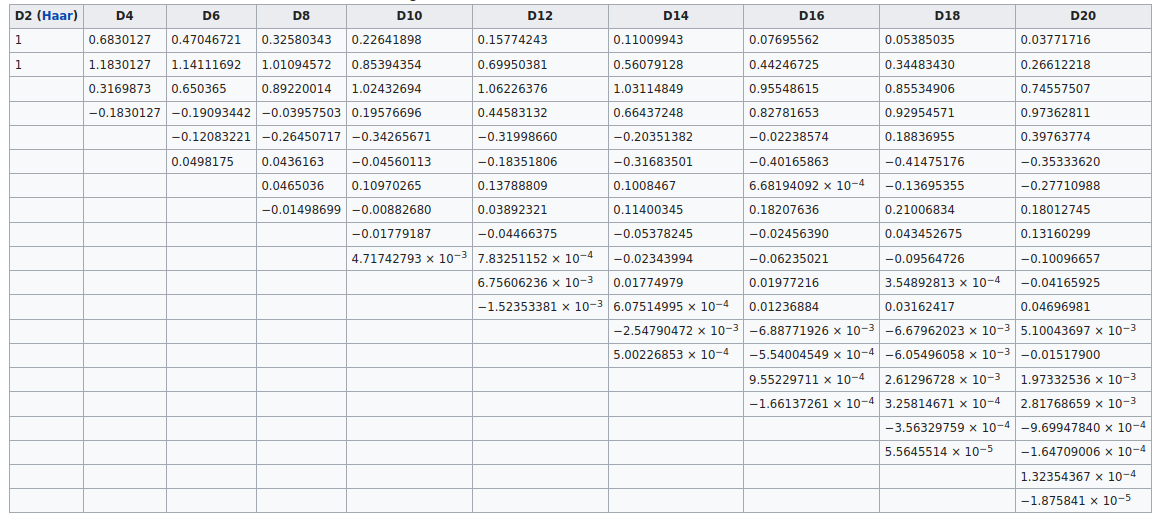
\includegraphics[scale=.35]{Graphics/Daubechies.png}
\caption{Coeficientes ortogonales de Daubechies.}
\label{coef-daubechies}
\end{figure}

\par Como se puede apreciar, las wavelets de Daubechies obtenidas ser\'an las mismas para un valor de $N$ dado y no se modificar\'an, independientemente de la se\~nal que se est\'e analizando. Si se desea realizar la tarea de detectar un patr\'on en una se\~nal no ser\'ia factible utilizar los mismos valores para cada muestra. Por ello, a la hora de construir una shapelet es necesario tener en cuenta la ``forma'' del patr\'on.

\par Las primeras dos condiciones correspondientes a la propiedad de ortogonalidad que deben cumplir los filtros (ecuaciones 1.1 y ~\ref{ortogonalidad}) son v\'alidas tambi\'en para las shapelets, pues son condiciones necesarias para que un conjunto de vectores sea considerado un banco de filtros.

\par En el caso de la tercera condici\'on, en vez de tener $\frac{N}{2}$ ecuaciones, se tomar\'an $\frac{N}{2}-2$ ecuaciones de momentos nulos. La raz\'on se debe a una cuarta condici\'on que requieren las shapelets. Supongase que se desea detectar un patr\'on $m$ y la informaci\'on que se conoce del mismo es que $m(k)=m_k$ para toda $k=0,1,\cdots,N$, las siguientes dos ecuaciones se conocen como ecuaciones de detecci\'on:
\begin{eqnarray}
\sum_{k=0}^{N}v(k)m(k)=0,
\label{matching1}\\
\sum_{k=0}^{N}v(k)m(k+1)=0.
\label{matching2}
\end{eqnarray}

\par A diferencia de las ecuaciones usadas en la DST-I, aqu\'i se consideran dos ecuaciones de detecci\'on debido a las traslaciones di\'adicas que sufre el filtro en la fase de an\'alisis de la se\~nal, que de usar una sola, podr\'ia provocar que no se detecte el patr\'on.\\

\par A continuaci\'on se muestra un ejemplo del m\'etodo propuesto. Se desea detectar el patr\'on de la Figura~\ref{patron-unidimensional} en una se\~nal de muestra, para ello es necesario determinar el banco de filtros de la shapelet correspondiente al patr\'on en cuesti\'on. Tomando $N=8$ se obtiene el siguiente sistema de ecuaciones no lineales:
\begin{eqnarray}
v(0)^2+v(1)^2+v(2)^2+v(3)^2+v(4)^2+v(5)^2+v(6)^2+v(7)^2=1,\nonumber
\end{eqnarray}
como condiciones de ortogonalidad las tres ecuaciones:
\begin{eqnarray}
v(0)v(2)+v(1)v(3)+v(2)v(4)+v(3)v(5)+v(4)v(6)+v(5)v(7)&=&0,\nonumber\\
v(0)v(4)+v(1)v(5)+v(2)v(6)+v(3)v(7)&=&0,\nonumber\\
v(0)v(6)+v(1)v(7)&=&0,\nonumber
\end{eqnarray}
dos ecuaciones de momentos nulos:
\begin{eqnarray}
v(0)+v(1)+v(2)+v(3)+v(4)+v(5)+v(6)+v(7)=0,\nonumber\\
v(1)+2v(2)+3v(3)+4v(4)+5v(5)+6v(6)+7v(7)=0,\nonumber
\end{eqnarray}
y dos ecuaciones de detecci\'on:
\begin{small}
\begin{eqnarray}
0.2v(0)+0.5v(1)+0.45v(2)+0.85v(3)+0.8v(4)-0.75v(5)+0.25v(6)+0.2v(7)=0,\nonumber\\
0.5v(0)+0.45v(1)+0.85v(2)+0.8v(3)-0.75v(4)+0.25v(5)+0.2v(6)+0.55v(7)=0.\nonumber
\end{eqnarray}
\end{small}

\begin{figure}[h]
\center
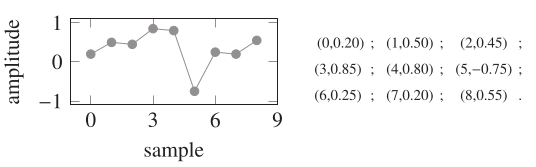
\includegraphics[scale=.5]{Graphics/Patron.png}
\caption{Ejemplo de una se\~nal patr\'on ($m$).}
\label{patron-unidimensional}
\end{figure}

\par Tras aplicar m\'etodos conocidos para la resoluci\'on de ecuaciones no lineales se obtiene como una de sus posibles soluciones:
\begin{eqnarray}
v = (-0.0834,0.1505,0.5719,-0.7055,-0.0091,-0.2784,0.2277,0.1263).\nonumber
\end{eqnarray}

\par Una vez obtenido $v$ es posible calcular el valor del resto de los filtros $u$, $\tilde{v}$ y $\tilde{u}$ que corresponden a los filtros de reconstrucci\'on pasa bajo, de an\'alisis pasa alto y an\'alisis pasa bajo respectivamente, de donde:

\begin{eqnarray}
u&=&(-0.1263,0.2277,0.2784,-0.0091,0.7055,0.5719,-0.1505,-0.0834),\nonumber\\
\tilde{v}&=&(-0.0834,0.1263,0.2277,-0.2784,-0.0091,-0.7055,0.5719,0.1505),\nonumber\\
\tilde{u}&=&(0.1505,-0.5719,-0.7055,0.0091,-0.2784,-0.2277,0.1263,0.0834).\nonumber
\end{eqnarray}

\par Al aplicar la transformada shapelet usando los filtros anteriores, se obtienen dos nuevos vectores $cA$ y $cD$ en la fase de an\'alisis que constituyen los coeficientes wavelets de la representaci\'on de la se\~nal original en la base $\{R_{2k}u\}_{k=0}^{\frac{N}{2}-1} \cup \{R_{2k}v\}_{k=0}^{\frac{N}{2}-1}$
\begin{eqnarray}
\left.\begin{array}{r}
D(z\ast\tilde{v})=cA\\
D(z\ast\tilde{u})=cD
\end{array}\right\}\mbox{fase de an\'alisis,}\nonumber
\end{eqnarray}
mientras que:
\begin{eqnarray}
\left.v\ast U(cA)+u\ast U(cD)=z\right\}\mbox{fase de s\'intesis.}\nonumber
\end{eqnarray}

\par El nuevo vector $cD$ es conocido en una dimensi\'on como el vector de detalles y es donde se almacenar\'an los valores que se necesitan para determinar la presencia o no del patr\'on que describen $u$ y $v$ dentro de la se\~nal. Para ello, se define una funci\'on de medida de similaridad $\mathbb{S}$ tal que $\mathbb{S}=e^{-\left|\mbox{\small{DST-II}}(z)\right|^{\alpha}}$, esta funci\'on enfatiza la presencia de ceros en el vector $\mbox{DST-II}(z)$ para un $0<\alpha<1$.

\par Sea la se\~nal de muestra de la Figura~\ref{signal-1d}, definida para toda $k\in \mathbb{Z}$ tal que $0\leq k \leq 63$:
\begin{eqnarray}
z(k)&=&\left\{\begin{array}{ll}
cos\left(\frac{27\pi k}{8}\right)sen\left(\frac{75\pi k}{8}\right),&\quad\mbox{para $0\leq k \leq 40$}\\
m(k),&\quad\mbox{para $41 \leq k \leq 49$}\\
cos\left(\frac{295\pi k}{32}\right)sen\left(\frac{105\pi k}{32}\right),&\quad\mbox{para $50 \leq k \leq 63$}
\end{array}\right.\nonumber
\end{eqnarray}

\begin{figure}[h]
\center
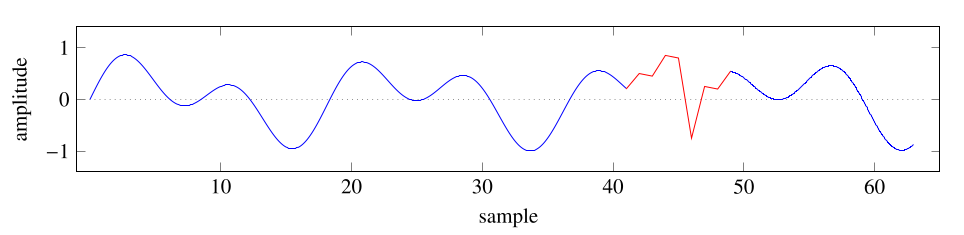
\includegraphics[scale=.4]{Graphics/Signal.png}
\caption{Se\~nal de muestra con el patr\'on $m$ incluido.}
\label{signal-1d}
\end{figure}

\par Sean $cA$ y $cD$ los vectores de aproximaci\'on y detalles, respectivamente obtenidos a partir de la DST-II. La figura~\ref{similaridad-1d} muestra los valores de estos vectores (naranja) y los valores de la medida de similaridad (azul, con $\alpha=0.1$) aplicada a cada uno de los valores de los vectores $cA$ y $cD$. Como se puede apreciar, para $k=53$ se obtiene un valor significativamente cercano a $1$ en el gr\'afico de similaridad, si se tiene en cuenta que, este valor corresponde al \'indice $k=21$ en el vector de aproximaci\'on $cD$ y, por tanto, a la posici\'on $k=42$ en la se\~nal original, entonces se puede afirmar que el algoritmo detect\'o satisfactoriamente al patr\'on $m$ en la se\~nal de muestra.

\begin{figure}[h]
\center
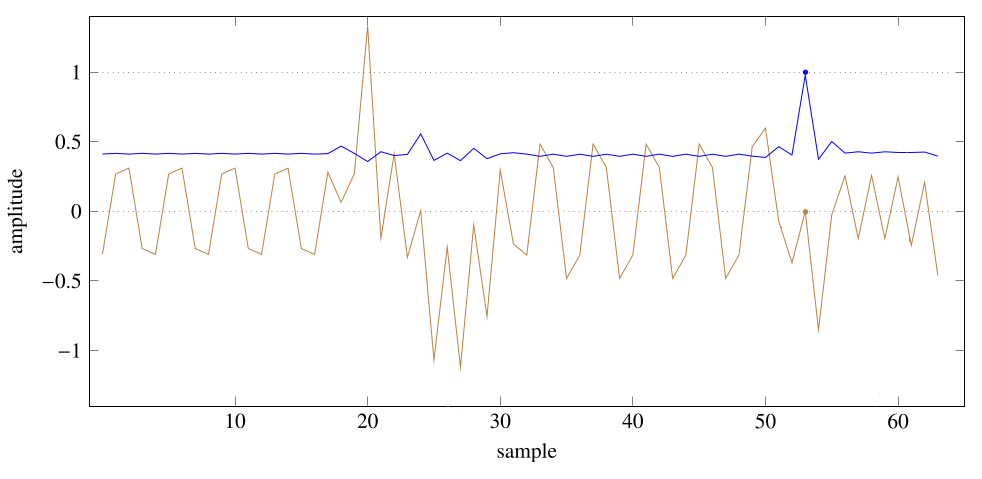
\includegraphics[scale=.4]{Graphics/Similarity.png}
\caption{Representaci\'on de los vectores de aproximaci\'on (los primeros 32 valores) y detalle (los valores entre 32 y 63) y, la medida de similaridad con el patr\'on.}
\label{similaridad-1d}
\end{figure}

\par Como parte del experimento, la medida $\mathbb{S}$ fue aplicada a los resultados obtenidos para los vectores $cA$ y $cD$ tras aplicar la transformada wavelet usando las wavelets: Haar, Daubechies 4, 6, 8, 10, 20, 30, 40, 50, 60 y 70, Symmlet 8 y 16, Coiflets 6, 12, 24, y 30, Beylkin 18 y, por \'ultimo, Vaidyanathan 24. Sin embargo DST-II fue la \'unica capaz de identificar al patr\'on $m$ dentro de la se\~nal $z$.

\section{Wavelets en dos dimensiones}\label{cap:w2d}

\par Hasta el momento se dispone de un m\'etodo para identificar un patr\'on dado en una se\~nal de muestra aplicando la transformada shapelet. Dicho m\'etodo funciona de manera efectiva en se\~nales unidimensionales, ?`que pasar\'ia entonces si se agrega una dimensi\'on m\'as? Para poder extender el concepto shapelet a dos dimensiones es necesario adaptar el conjunto de herramientas del cual se dispone en una dimensi\'on a dos dimensiones, tal que sea capaz de obtener similares resultados ya no solo para se\~nales sino tambi\'en para im\'agenes.\\

\par Anteriormente, se dieron un conjunto de definiciones para mostrar un algoritmo que permitiera, a partir de un vector, construir un banco de filtros y, por consiguiente, una base wavelet. Una imagen puede ser representada por un vector en $\ell^2(\mathbb{Z}_{N_1}\times\mathbb{Z}_{N_2})$, donde $\ell^2(\mathbb{Z}_{N_1}\times\mathbb{Z}_{N_2})=\{z(i,j)|0\leq i \leq N_1-1,\,0\leq j\leq N_2-1\}$, consid\'erese entonces dicho espacio como el punto de partida.

\subsection{Definiciones}

\par Las siguientes definiciones fueron extra\'idas de [\textcolor{cyan}{\cite{12}}].\\

\begin{definition}
Para $z\in \ell^2(\mathbb{Z}_{N_1}\times\mathbb{Z}_{N_2})$ se define $\hat{z}$ como la transformada discreta de Fourier de $z$ tal que:
\begin{eqnarray}
\hat{z}(m_1,m_2)&=&\sum_{n_1=0}^{N_1-1}\sum_{n_2=0}^{N_2-1}z(n_1,n_2)e^{\frac{-2\pi im_1n_1}{N_1}}e^{\frac{-2\pi im_2n_2}{N_2}},\qquad\forall\,m_1,m_2.\nonumber
\end{eqnarray}
\end{definition}

\begin{definition}
Para $z\in \ell^2(\mathbb{Z}_{N_1}\times\mathbb{Z}_{N_2})$ se define $\tilde{z}$ como la reflexi\'on conjugada de $z$ tal que:
\begin{eqnarray}
\tilde{z}(m_1,m_2)&=&\overline{z(-m_1,-m_2)}=\overline{z(N_1-m_1,N_2-m_2)},\qquad\forall\,m_1,m_2.\nonumber
\end{eqnarray}
\end{definition}

\begin{definition}
Para todo $w,z\in \ell^2(\mathbb{Z}_{N_1}\times\mathbb{Z}_{N_2})$ se define la convoluci\'on entre ellos como $z\ast w$ tal que:
\begin{eqnarray}
(z\ast w)(m_1,m_2)&=&\sum_{n_1=0}^{N_1-1}\sum_{n_2=0}^{N_2-1}z(m_1-n_1,m_2-n_2)w(n_1,n_2),\qquad\forall\,m_1,m_2.\nonumber
\end{eqnarray}
\end{definition}

\begin{definition}
Para $z\in \ell^2(\mathbb{Z}_{N_1}\times\mathbb{Z}_{N_2})$ y $k_1,k_2\in\mathbb{Z}$ se define $R_{k_1,k_2}{z}$ como la traslaci\'on de $z$ por $k_1,k_2$ dado por:
\begin{eqnarray}
R_{k_1,k_2}{z}(m_1,m_2)&=&z(m_1-k_1,m_2-k_2),\qquad\forall\,m_1,m_2.\nonumber
\end{eqnarray}
\end{definition}

\subsection{Banco de filtros}

\begin{theorem}
(Ver demostraci\'on en [\textcolor{cyan}{\cite{12}}]) Sup\'ongase que $M_1,M_2\in\mathbb{N}$, $N_1=2M_1$, $N_2=2M_2$ y $u_1,u_2\in \ell^2(\mathbb{Z}_{N_1}\times\mathbb{Z}_{N_2})$. Entonces, para todo $0\leq k_1 \leq M_1-1$ y\linebreak $0\leq k_2 \leq M_2-1$, $\{R_{2k_1,2k_2}u_1\}$ y $\{R_{2k_1,2k_2}u_2\}$ son conjuntos biortonormales si y solo si:
\begin{eqnarray}
u^1+u^2+u^3+u^4&=&4,\nonumber
\end{eqnarray}
donde
\begin{eqnarray}
u^1&=&\hat{u_1}(n_1,n_2)\overline{\hat{u_2}(n_1,n_2)},\nonumber\\
u^2&=&\hat{u_1}(n_1+M_1,n_2)\overline{\hat{u_2}(n_1+M_1,n_2)},\nonumber\\
u^3&=&\hat{u_1}(n_1,n_2+M_2)\overline{\hat{u_2}(n_1,n_2+M_2)},\nonumber\\
u^4&=&\hat{u_1}(n_1+M_1,n_2+M_2)\overline{\hat{u_2}(n_1+M_1,n_2+M_2)}.\nonumber
\end{eqnarray}
\end{theorem}

\begin{theorem}
(Ver demostraci\'on en [\textcolor{cyan}{\cite{12}}]) Sup\'ongase que $M_1,M_2\in\mathbb{N}$, $N_1=2M_1$, $N_2=2M_2$ y $u_i,v_i\in \ell^2(\mathbb{Z}_{N_1}\times\mathbb{Z}_{N_2})$, para toda $i=0,1,2,3$. Entonces, para todo\linebreak $0\leq k_1 \leq M_1-1$ y $0\leq k_2 \leq M_2-1$,
\begin{eqnarray}
\bigcup_{m=0}^{3}\{R_{2k_1,2k_2}u_m\}\mbox{ y }\bigcup_{m=0}^{3}\{R_{2k_1,2k_2}v_m\},\nonumber
\end{eqnarray}
son conjuntos biortogonales de $\ell^2(\mathbb{Z}_{N_1}\times\mathbb{Z}_{N_2})$ si y solo si:
\begin{eqnarray}
A_u(n_1,n_2)^T\overline{A_v(n_1,n_2)}=\left[\begin{array}{cccc}
1&0&0&0\\0&1&0&0\\0&0&1&0\\0&0&0&1
\end{array}\right],\nonumber
\end{eqnarray}
para todo $0\leq n_1 \leq M_1-1$, $0\leq n_2 \leq M_2-1$, donde $A_u(n_1,n_2)$ es la matriz cuya $m-$\'esima columna ($m=0,1,2,3$) es:
\begin{eqnarray}
\frac{1}{2}\left[\begin{array}{c}
\hat{u}_m(n_1,n_2)\\
\hat{u}_m(n_1+M_1,n_2)\\
\hat{u}_m(n_1,n_2+M_2)\\
\hat{u}_m(n_1+M_1,n_2+M_2)
\end{array}\right],\nonumber
\end{eqnarray}
y $A_v(n_1,n_2)$ es la matriz cuya $m-$\'esima columna ($m=0,1,2,3$) es:
\begin{eqnarray}
\frac{1}{2}\left[\begin{array}{c}
\hat{v}_m(n_1,n_2)\\
\hat{v}_m(n_1+M_1,n_2)\\
\hat{v}_m(n_1,n_2+M_2)\\
\hat{v}_m(n_1+M_1,n_2+M_2)
\end{array}\right].\nonumber
\end{eqnarray}
\label{biortogonalidad}
\end{theorem}

\begin{definition}
Suponga que $M_1,M_2\in\mathbb{N}$, $N_1=2M_1$ y $N_2=2M_2$. Se definen los operadores $$D^l: \ell^2(\mathbb{Z}_{N_1}\times\mathbb{Z}_{N_2})\rightarrow \ell^2\left(\mathbb{Z}_{\frac{N_1}{2^l}}\times\mathbb{Z}_{\frac{N_2}{2^l}}\right),$$ de submuestreo y $$U^l: \ell^2\left(\mathbb{Z}_{\frac{N_1}{2^l}}\times\mathbb{Z}_{\frac{N_2}{2^l}}\right)\rightarrow \ell^2(\mathbb{Z}_{N_1}\times\mathbb{Z}_{N_2}),$$ de sobremuestreo como:
\begin{eqnarray}
D^l(z)(n_1,n_2)=z(2^ln_1,2^ln_2),\qquad\forall\,z\in \ell^2(\mathbb{Z}_{N_1}\times\mathbb{Z}_{N_2}),\nonumber
\end{eqnarray}
y
\begin{eqnarray}
U^l(z)(n_1,n_2)&=&\left\{\begin{array}{rr}
z\left(\frac{n_1}{2^l},\frac{n_2}{2^l}\right),&\quad 2^l | n_1,\, 2^l|n_2\\
0,&\quad\mbox{en otro caso,}
\end{array}\right.\nonumber\\
\forall\,z&\in &\ell^2\left(\mathbb{Z}_{\frac{N_1}{2^l}}\times\mathbb{Z}_{\frac{N_2}{2^l}}\right),\nonumber
\end{eqnarray}
donde $D^1=D$, $U^1=U$ y $D^l(z)=(D\circ D^{l-1})(z)$, $U^l(z)=(U\circ U^{l-1})(z)$ para $l>1$.
\end{definition}

\begin{theorem}
(Ver demostraci\'on en [\textcolor{cyan}{\cite{12}}]) Sup\'ongase que $M_1,M_2\in\mathbb{N}$, $N_1=2M_1$, $N_2=2M_2$ y $u_0,u_1,u_2,u_3,s_0,s_1,s_2,s_3\in \ell^2(\mathbb{Z}_{N_1}\times\mathbb{Z}_{N_2})$. Sea la matriz $A(n_1,n_2)$ definida como en el Teorema 1.2, entonces se tiene una reconstrucci\'on perfecta:
\begin{eqnarray}
\sum_{i=0}^3 \tilde{s}_i\ast U(D(z\ast\tilde{u}_i))=z,\nonumber
\end{eqnarray}
para toda $z\in \ell^2(\mathbb{Z}_{N_1}\times\mathbb{Z}_{N_2})$, si y solo si:
\begin{eqnarray}
A(n_1,n_2)\left[\begin{array}{c}
\hat{s}_0\\ \hat{s}_1\\ \hat{s}_2\\ \hat{s}_3
\end{array}\right]=\left[\begin{array}{c}
2\\0\\0\\0
\end{array}\right],\nonumber
\end{eqnarray}
para todo $n_1,n_2$. En el caso de que $A(n_1,n_2)$ sea unitaria, entonces $s_i=\tilde{u}_i$ para $i=0,1,2,3$.
\label{reconstruccion-perfecta}
\end{theorem}

\par De los teoremas 1.2 y 1.3 se sabe que si:
\begin{eqnarray}
\bigcup_{m=0}^{3}\{R_{2k_1,2k_2}u_m\},\nonumber
\end{eqnarray}
es un conjunto biortogonal consigo mismo en $\ell^2(\mathbb{Z}_{N_1}\times\mathbb{Z}_{N_2})$ entonces la matriz $A(n_1,n_2)$ es unitaria y, por tanto:
\begin{eqnarray}
\sum_{i=0}^3 u_i\ast U(D(z\ast\tilde{u}_i))=z,\nonumber
\end{eqnarray}
constituye una reconstrucci\'on perfecta de una imagen $z$. Esto quiere decir que al igual que en una sola dimensi\'on, el problema de crear una base wavelet que permita detectar un patr\'on, se reduce al c\'alculo efectivo de un banco de filtros $\{u_i\}\cup\{\tilde{u}_i\}$, ahora biortogonal. Este constituye el pr\'oximo paso en la tarea de crear una shapelet de dos dimensiones.\\